\documentclass{beamer}
\mode<presentation>
\usepackage{amsmath}
\usepackage{amssymb}
%\usepackage{advdate}
\usepackage{adjustbox}
\usepackage{subcaption}
\usepackage{enumitem}
\usepackage{multicol}
\usepackage{mathtools}
\usepackage{listings}
\usepackage{url}
\def\UrlBreaks{\do\/\do-}
\usetheme{Boadilla}
\usecolortheme{lily}
\setbeamertemplate{footline}
{
  \leavevmode%
  \hbox{%
  \begin{beamercolorbox}[wd=\paperwidth,ht=2.25ex,dp=1ex,right]{author in head/foot}%
    \insertframenumber{} / \inserttotalframenumber\hspace*{2ex} 
  \end{beamercolorbox}}%
  \vskip0pt%
}
\setbeamertemplate{navigation symbols}{}

\providecommand{\nCr}[2]{\,^{#1}C_{#2}} % nCr
\providecommand{\nPr}[2]{\,^{#1}P_{#2}} % nPr
\providecommand{\mbf}{\mathbf}
\providecommand{\pr}[1]{\ensuremath{\Pr\left(#1\right)}}
\providecommand{\qfunc}[1]{\ensuremath{Q\left(#1\right)}}
\providecommand{\sbrak}[1]{\ensuremath{{}\left[#1\right]}}
\providecommand{\lsbrak}[1]{\ensuremath{{}\left[#1\right.}}
\providecommand{\rsbrak}[1]{\ensuremath{{}\left.#1\right]}}
\providecommand{\brak}[1]{\ensuremath{\left(#1\right)}}
\providecommand{\lbrak}[1]{\ensuremath{\left(#1\right.}}
\providecommand{\rbrak}[1]{\ensuremath{\left.#1\right)}}
\providecommand{\cbrak}[1]{\ensuremath{\left\{#1\right\}}}
\providecommand{\lcbrak}[1]{\ensuremath{\left\{#1\right.}}
\providecommand{\rcbrak}[1]{\ensuremath{\left.#1\right\}}}
\theoremstyle{remark}
\newtheorem{rem}{Remark}
\newcommand{\sgn}{\mathop{\mathrm{sgn}}}
\providecommand{\abs}[1]{\left\vert#1\right\vert}
\providecommand{\res}[1]{\Res\displaylimits_{#1}} 
\providecommand{\norm}[1]{\lVert#1\rVert}
\providecommand{\mtx}[1]{\mathbf{#1}}
\providecommand{\mean}[1]{E\left[ #1 \right]}
\providecommand{\fourier}{\overset{\mathcal{F}}{ \rightleftharpoons}}
%\providecommand{\hilbert}{\overset{\mathcal{H}}{ \rightleftharpoons}}
\providecommand{\system}{\overset{\mathcal{H}}{ \longleftrightarrow}}
	%\newcommand{\solution}[2]{\textbf{Solution:}{#1}}
%\newcommand{\solution}{\noindent \textbf{Solution: }}
\providecommand{\dec}[2]{\ensuremath{\overset{#1}{\underset{#2}{\gtrless}}}}
\newcommand{\myvec}[1]{\ensuremath{\begin{pmatrix}#1\end{pmatrix}}}
\let\vec\mathbf

\lstset{
%language=C,
frame=single, 
breaklines=true,
columns=fullflexible
}

\numberwithin{equation}{section}

\title{Area between two curves by using matrix method}
\author{Prajwal \\EE24BTECH11051 \\ Electrical Enggineering ,\\IIT Hyderabad.}

\date{\today} 
\begin{document} 

\begin{frame}
\titlepage
\end{frame}

\section*{Outline}
\begin{frame}
\tableofcontents
\end{frame}
\section{Problem}
\begin{frame}
\frametitle{Problem Statement}

Using integration, find the area of the region bounded by the parabolas $y^2\;=\;4x$ and  $x^2\;=\;4y$.
\\ \begin{table}[h!]    
  \centering
  \begin{center}
    \begin{tabular}{|c|c|c|} 
        \hline
            \textbf{Variable} & \textbf{Description} & \textbf{Formula} \\ 
        \hline
            $A$   & It is one end of the line segment & $\myvec{5 \\ -6}$ \\ 
        \hline
            $B$   & It is other end of line segment &  $\myvec{-1\\-4}$\\ 
        \hline
            $C$   & It is the point of intersection of line segment and $Y$-axis & $C  = \myvec{0\\y}$\\ 
        \hline
        
    \end{tabular}
\end{center}  

  \caption{Variables Used}
\end{table}
\end{frame}
\section{Solution}
\subsection{Conic Parameters}
\begin{frame}
\frametitle{Conic Parameters}
%\framesubtitle{Literature}
 The conic parameters of circle $y^2=4x$ are :
 \begin{center}
      $V_1 = \myvec{ 0 &0\\ 0 &1}, u_1 =\myvec{-2 \\ 0}, f_1 = 0 $
 \end{center}
 Conic parameters of parabola $x^2=4y$ can be expressed as :
 \begin{center}
      $V_2 = \myvec{ 1 &0\\ 0 &0}, u_2 =\myvec{0 \\ -2}, f_2 = 0$
 \end{center}
 
\end{frame}
\subsection{Intersection of conics}
\begin{frame}
\frametitle{Intersection of conics}
The intersection of two conics with parameters$ V_i, u_i, f_i (i = 1, 2) $is defined as :
\begin{center}
    $x^\top (V_1 + \mu V_2) x + 2(u_1 + \mu u_2)^\top x + (f_1 + \mu f_2) = 0$
\end{center}
On solving we get the points of intersection are :
\begin{center}
    $\myvec{0\\0}\;,\myvec{4\\4}$
\end{center}
\end{frame}
\subsection{Area calculation}
\begin{frame}
\frametitle{Area calculation}
Area between the curves is,
\begin{align}
2\int_{0}^{4} \brak{\sqrt{4x}-\frac{x^2}{4}} \, dy 
\end{align}
By solving the integration, we get area is equal to 5.33 sq.units
\end{frame}
\subsection{Figure}
\begin{frame}
\frametitle{Figure}
\begin{figure}
   \centering
   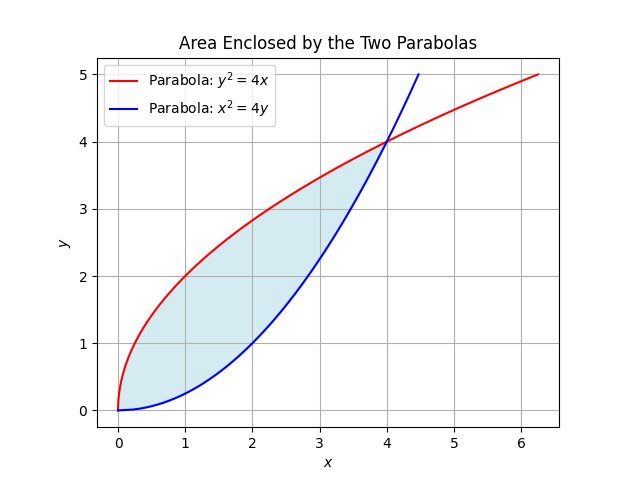
\includegraphics[width=\linewidth]{figs/Figure_1.png}
   \label{stemplot}
   \caption{}
\end{figure}
\end{frame}
\section{C Code}
\begin{frame}[fragile]
\frametitle{C Code }
\begin{lstlisting}[language=C]
#include <stdio.h>

int main() {
    // Define parabola parameters
    double p1 = 1.0; // Parameter for y^2 = 4px
    double p2 = 1.0; // Parameter for x^2 = 4py

    // Open the file to write the parameters
    FILE *file = fopen("data.txt", "w");
    if (file == NULL) {
        printf("Error opening file!\n");
        return 1;
        }
    
\end{lstlisting}
\end{frame}

\begin{frame}[fragile]
\begin{lstlisting}[language=C]

    // Write the parabola parameters to the file
    fprintf(file, "%f\n", p1); // Parameter for the first parabola
    fprintf(file, "%f\n", p2); // Parameter for the second parabola

    // Close the file
    fclose(file);

    printf("Data written to data.txt\n");

    return 0;
}
    
\end{lstlisting}
\end{frame}
\section{Python Code}
\begin{frame}[fragile]
\frametitle{Python Code for Plotting}
\begin{lstlisting}[language=Python]

import numpy as np
import matplotlib.pyplot as plt
from scipy.integrate import quad
from scipy.optimize import fsolve

# Read the values from the C-generated text file using numpy.loadtxt
data = np.loadtxt('data.txt')

# Extracting parabola parameters
p1 = data[0]  # Parameter for y^2 = 4x
p2 = data[1]  # Parameter for x^2 = 4y

# Parabola equation: y^2 = 4px, so x = y^2 / (4p)
def parabola1(y, p):
    return y**2 / (4 * p)


\end{lstlisting}
\end{frame}
\begin{frame}[fragile]
\begin{lstlisting}[language=Python]
def parabola2(x, p):
    return x**2 / (4 * p)

# Find the points of intersection between the two parabolas
def find_intersections(p1, p2):
    def intersection_eq(y):
        return parabola2(parabola1(y, p1), p2) - y  # Solve for intersection

    y_int1 = fsolve(intersection_eq, 0)[0]  # Initial guess
    y_int2 = fsolve(intersection_eq, 4)[0]  # Initial guess for the other intersection
    return y_int1, y_int2

# Get the intersection points
y_int1, y_int2 = find_intersections(p1, p2)

  
\end{lstlisting}
\end{frame}
\begin{frame}[fragile]
\begin{lstlisting}[language=Python]
# Compute the area between the curves using integration
def area_between_curves(y):
    x1 = parabola1(y, p1)  # x from the first parabola
    x2 = 2 * np.sqrt(y)  # From the second parabola (x = 2*sqrt(y))
    return x2 - x1  # Area between the two parabolas

# Perform the integration from y_int1 to y_int2
area, _ = quad(area_between_curves, y_int1, y_int2)



# Visualization
# Generating points for the parabolas
y_vals = np.linspace(0, y_int2 + 1, 400)  # Extend range a bit above the highest intersection
x_parabola1 = parabola1(y_vals, p1)
x_parabola2 = 2 * np.sqrt(y_vals)  # From the second parabola
\end{lstlisting}
\end{frame}
\begin{frame}[fragile]
\begin{lstlisting}[language=Python]
# Plot the curves
plt.plot(x_parabola1, y_vals, label=r'Parabola: $y^2 = 4x$', color='r')
plt.plot(x_parabola2, y_vals, label=r'Parabola: $x^2 = 4y$', color='b')

# Fill the area between the curves
plt.fill_betweenx(y_vals, x_parabola1, x_parabola2, where=(x_parabola2 >= x_parabola1), color='lightblue', alpha=0.5)

# Labels and plot settings
plt.xlabel('$x$')
plt.ylabel('$y$')
plt.title('Area Enclosed by the Two Parabolas')
plt.grid(True)
plt.legend()
\end{lstlisting}
\end{frame}
\begin{frame}[fragile]
\begin{lstlisting}[language=Python]
# Set equal aspect ratio to avoid distortion
plt.gca().set_aspect('equal', adjustable='box')

# Show the plot
plt.show()
\end{lstlisting}
\end{frame}
\end{document}
